\chapter{Introduction to data}
\label{introductionToData}

\section{Continuous and discrete}
The distinction between continuous and discrete data is common in mathematics. \emph{Continuous} refers to real numbers drawn from the set of all such, $\mathbb R$. \emph{Discrete} refers to a finite or countably infinite set such as the natural numbers $\mathbb N$.

If salaries are measured in integer multiples of \$100, they can be considered discrete; in fact, a salary is presumably always an integer multiple of 1 cent. However, it is somewhat artificial to consider a salary as discrete, as only convenience stops us from using salaries involving fractions of a cent.

\begin{example}{Impossible salaries}
	Estelle has \$100,000 to spend on salaries for three employees. Since the employees are indistinguishable, other things being equal, she decides to give them each a salary of
	\[
		\$\frac{100,000}3.
	\]
\end{example}

\begin{example}{Discrete time?}%Austin
	Time is usually measured in real numbers, although it is not known for sure in theoretical physics whether
	time is actually discrete\footnote{\url{https://physics.stackexchange.com/questions/35674/is-time-continuous-or-discrete}}.
	This would mean that there is a limit to how small time steps one can take.
\end{example}

\section{Categorical variables}
Within categorical variables, the ordinal ones are ordered. Note that one can imagine variables whose values are structured, without being numeric or ordinal: for instance, consider \var{direction}:
\begin{quote}
	 North,
	 Northwest,
	 West,
	 Southwest,
	 South,
	 Southeast,
	 East,
	 Northeast.
\end{quote}
These are naturally ordered in a circle or loop.

\begin{exercise} %\index{data!stroke}
What could be another example of a structured variable, which is nevertheless not numerical or ordinal?
Maybe another variable that is naturally ordered in a ``wheel''?\footnote{How about a kids' favorite: color. Colors are ordered cyclically as
 \begin{quote}
	 Red,
	 Orange,
	 Yellow,
	 Green,
	 Blue,
	 Purple.
 \end{quote}
}
\end{exercise}

\begin{exercise}%Thanks to Spencer.
	What kind of mathematical structure can you find in the variable ``state of residence'' among the U.S.~states?\footnote{For instance, consider whether two states are neighbors; this will give a graph structure as studied in discrete mathematics.}
\end{exercise}

\section[Examining numerical data]{Examining numerical data}
\label{numericalData}

\begin{termBox}{\tBoxTitle{Mean}%
The sample mean of a numerical variable is computed as the sum of all of the observations divided by the number of observations:
\begin{eqnarray}
\bar{x} = \frac{x_1+x_2+\cdots+x_n}{n}
\label{meanEquation}
\end{eqnarray}
where $x_1, x_2, \dots, x_n$ represent the $n$ observed values.}
\end{termBox}\marginpar[\raggedright\vspace{-8mm}

$n$\\\footnotesize sample size]{\raggedright\vspace{-8mm}

$n$\\\footnotesize sample size}\vspace{-2mm}

%The above is a special trick to make text appear in the margin!

This arithmetic mean has a very important property: suppose you want to load goods onto a ship, airplane, or car. If you know the mean weight of the goods, and you know how many there are of them, then you know the total weight. Some other kinds of ``mean'' are developed in Exercise \ref{harmonic}. The geometric mean studied there could be similarly applied: if you know the geometric mean of the factors by which a stock price changes, and you know the number of changes, then you know the overall change.


A \term{mode} is represented by a prominent peak in the distribution. To be mathematically precise, we could let the mode be the value with the most occurrences. But it is common to have \emph{no} observations with the same value in a data set, which makes this other definition useless for many real data sets. See Chapter 2 for a definition of mode in that case.

\label{variability}

We define as follows the sample \term{variance}\label{varianceIsDefined}, denoted by $s_{}^2$\marginpar[\raggedright$s^2_{}$\\\footnotesize sample variance]{\raggedright$s^2_{}$\\\footnotesize sample variance}:
\begin{align*}
s_{}^2 = \frac1{n-1}\sum_{i=1}^n (x_i-\overline x)^2
\end{align*}
We divide by $n-1$, rather than dividing by $n$. To see why, consult Chapter 2. The \term{sample standard deviation} is then $s=\sqrt{s^2}$.

The reason for using squares rather than, say, fourth powers in the definition of variance is related to Pythagoras Theorem and ideas about orthogonality.
It turns out that for random variables $X$ and $Y$ that are independent (which is analogous to orthogonal), we have $\Var(X+Y)=\Var(X)+\Var(Y)$, analogously to how if $a$ and $b$ are side lengths of orthogonal sides in a triangle, then the length of the hypotenuse is $\sqrt{a^2+b^2}$.

The standard deviation has an advantage over the variance in that, when used in physical examples, it has the same physical units as the original data. This also means that it should make sense to add a fixed number of standard deviations to the data points (where it would make little sense too a number of variances).

Would it make sense to consider, say, twice the standard deviation $2\sigma$ instead of the standard deviation $\sigma$? Yes, and in fact there is a vigorous debate in some circles about the merits of $pi=3.14\dots$ versus $\tau=2\pi$. In the normal probability density function, there is a factor $\sqrt{2\pi}\sigma$, so that arguably it would look simpler if we used $\sqrt{2\pi}\sigma$ instead of $\sigma$. At some point, we just have to assert that what constant to put in front is a matter of convention.

\subsection{About those pie charts}
A \term{pie chart} is shown in Figure~\vref{emailNumberPieChart} alongside a bar plot.
The much maligned pie charts are actually useful when you want to see at a glance if a proportion is close to 50\% or 25\%.

\begin{figure}[h]
   \centering
   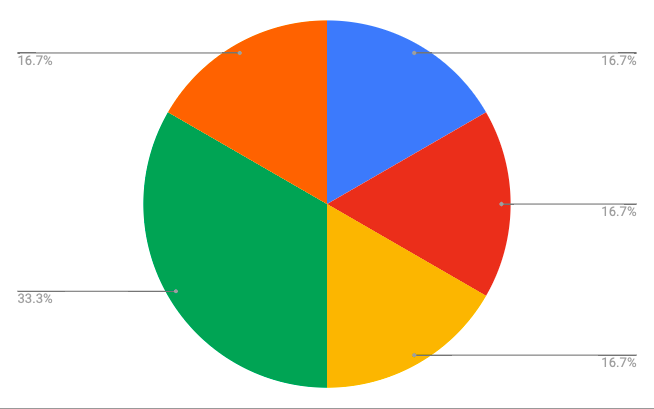
\includegraphics[width=0.5\textwidth]{ch_intro_to_data/figures/pie-chart-s4cs}
   \caption{A pie chart for the data 1,1,1,2,1.}
   \label{emailNumberPieChart}
\end{figure}

\begin{exercise}
	Could any other shapes than discs be as useful for ``pie'' charts?\footnote{A hexagonal chart could be useful for identifying whether a proportion was greater than $1/6$, for instance.}
\end{exercise}

\section{Sampling}

This topic is treated extensively in \emph{OpenIntro Statistics} and we confine ourselves to some remarks.

A \emph{simple random sample} is one in which each set of $n$ outcomes is equally likely to appear.
For instance, if we sample $n=2$ individuals from $\{1,2,3\}$, we would need to know that $\{1,2\}$, $\{2,3\}$, and $\{1,3\}$ are equally likely. It is not enough that, say, 1, 2, and 3 each have probability $1/3$ of appearing in our set.

If two samples of individuals are drawn from the same distribution, but then we \emph{treat} the individuals in two different ways, we are \emph{causing} a change and can conclude that, most likely, any difference in the results for the two samples was \emph{caused} by our treatment. For observational studies we must always worry that there may be other explanations. Suppose countries with a lot of pianos also have low rates of malnutrition. We cannot conclude that there is a causal relationship. In this example it seems silly to think there would be one.

%\begin{exercise}
%Is blocking basically the same as stratified sampling, except that blocking is used for experiments?\footnote{It seems so, although different authors may use these words slightly differently.}
%\end{exercise}

